%
% fig/napoleon.tex -- Napoleon-Dreieck am konkreten Beispiel
% A = 8 + 20i, B = 28 + 22i, C = 17 + 25i (gemaess Praesentation).
% Wir verschieben den Schwerpunkt in den Ursprung und skalieren mit 0.2,
% damit das Bild auf die Seite passt.
%
\begin{figure}
\centering
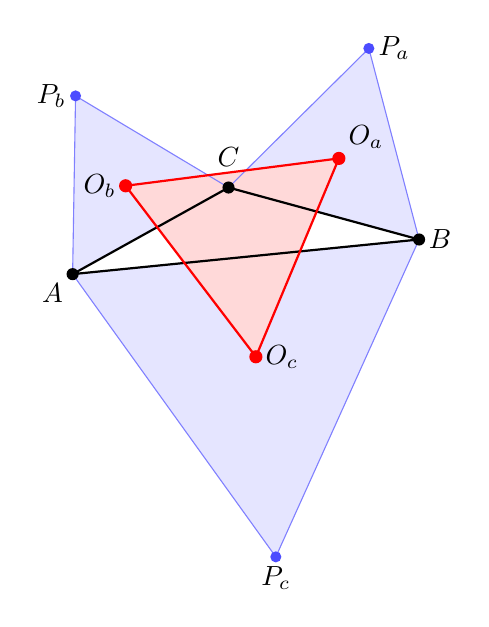
\begin{tikzpicture}[>=latex,scale=0.22]
% Ausgangsdreieck ABC (Originalkoordinaten aus Praesentation)
\coordinate (A)  at ( 8, 20);
\coordinate (B)  at (28, 22);
\coordinate (C)  at (17, 25);
% Aussen errichtete Eckpunkte
\coordinate (Pa) at (25.10, 33.03);  % gegenueber A, ueber BC
\coordinate (Pb) at ( 8.17, 30.29);  % gegenueber B, ueber CA
\coordinate (Pc) at (19.73,  3.68);  % gegenueber C, ueber AB
% Schwerpunkte der drei aussen errichteten Dreiecke
\coordinate (Oa) at (23.37, 26.68);
\coordinate (Ob) at (11.06, 25.10);
\coordinate (Oc) at (18.58, 15.23);
% Aussen errichtete gleichseitige Dreiecke (ausgefuellt schwach)
\fill[blue!10] (B) -- (C) -- (Pa) -- cycle;
\fill[blue!10] (C) -- (A) -- (Pb) -- cycle;
\fill[blue!10] (A) -- (B) -- (Pc) -- cycle;
% Schwerpunktdreieck (rot ausgefuellt)
\fill[red!15] (Oa) -- (Ob) -- (Oc) -- cycle;
% Konturen der aussen errichteten Dreiecke
\draw[blue!50,thin] (B) -- (Pa) -- (C);
\draw[blue!50,thin] (C) -- (Pb) -- (A);
\draw[blue!50,thin] (A) -- (Pc) -- (B);
% Ausgangsdreieck (kraeftig schwarz)
\draw[thick] (A) -- (B) -- (C) -- cycle;
% Schwerpunktdreieck (kraeftig rot)
\draw[red,thick] (Oa) -- (Ob) -- (Oc) -- cycle;
% Punkte
\foreach \p in {A,B,C} \fill (\p) circle (0.35);
\foreach \p in {Pa,Pb,Pc} \fill[blue!70] (\p) circle (0.32);
\foreach \p in {Oa,Ob,Oc} \fill[red] (\p) circle (0.38);
% Beschriftungen
\node at (A)  [below left]  {$A$};
\node at (B)  [right]       {$B$};
\node at (C)  [above,yshift=4pt] {$C$};
\node at (Pa) [right]       {$P_a$};
\node at (Pb) [left]        {$P_b$};
\node at (Pc) [below]       {$P_c$};
\node at (Oa) [above right] {$O_a$};
\node at (Ob) [left]        {$O_b$};
\node at (Oc) [right]       {$O_c$};
\end{tikzpicture}
\caption{Konstruktion zum Satz von Napoleon am Beispiel
$A = 8 + 20i$, $B = 28 + 22i$, $C = 17 + 25i$.
Über jeder Seite des Ausgangsdreiecks $ABC$ (schwarz) wird ein
gleichseitiges Dreieck nach aussen errichtet (blau).
Die Schwerpunkte $O_a$, $O_b$, $O_c$ dieser drei aussen errichteten
Dreiecke bilden das Napoleon-Dreieck (rot), das stets gleichseitig ist.
\label{komplex:figure:napoleon}}
\end{figure}
